\documentclass[11pt]{article}

%Afegim els "packages" necessaris per generar el document

\usepackage[utf8]{inputenc}
\usepackage[catalan]{babel}
\selectlanguage{catalan}

\usepackage{graphicx}
\usepackage{fancyhdr}
\usepackage{hyperref}
\usepackage{tocloft}
\usepackage[T1]{fontenc}


\title{Instal·lació Code-Lite + Allegro 5.1 (Windows)}
\author{Autor: Albert Lloveras Carbonell\\Revisió: Joaquim Porte Rodríguez}
\date{}

\renewcommand\contentsname{\huge Índex \vspace{8pt} \hrule}
\renewcommand{\cftsecleader}{\cftdotfill{\cftdotsep}}

%------------------------------------------------------------
%	Definició de Capçaleres i Peus de Pàgina
%------------------------------------------------------------

\fancypagestyle{pageStyle}{
	%Definim la capçalera de l'esquerra (Logo Salle)
	\fancyhead[L]{
		
\includegraphics[scale=0.25]{img/la_salle_logo.jpg}
	} 

	%Definim la capçalera de la dreta (Info Curs i Assignatura)
	\fancyhead[R]{
		\vtop{
			Manual d'instal·lació\\
			Code-Lite + Allegro5.1 (Windows)\\
		}
	}
	\fancyfoot[C]{} %Peu de pàgina central
	\fancyfoot[L]{Departament d'Enginyeria - Informàtica} %Peu de pàgina esquerra
	\fancyfoot[R]{\thepage} %Peu de pàgina dreta (Número de pàgina)	
	%Configuracions extra
	\renewcommand{\headrulewidth}{0pt} %Ocultem la línia de separació entre 		capçalera i bloc de text
	\renewcommand{\footrulewidth}{2pt} %Fixem la línia de separació entre peu de pàgina i bloc de text
	\setlength{\headheight}{67pt} %Fixem la mida de la capçalera	
	
}

%Definim la macro (nofooter) per poder amagar el peu de pàgina quan interessi
\fancypagestyle{nofooter}{
	\fancyfoot{}
	\renewcommand{\footrulewidth}{0pt}
}

%Definim la macro (nofooter) per poder amagar el peu de pàgina quan interessi
\fancypagestyle{empty}{
	\fancyfoot{}
	\fancyhead{}
	\renewcommand{\footrulewidth}{0pt}
	\renewcommand{\headrulewidth}{0pt}
}

\begin{document}

\pagestyle{empty}
\begin{center}

	%--- Logo de la portada --- %
	
\includegraphics[width=0.15\textwidth]{img/code-lite.png}~\\[1cm]
	
	%---- Nom del programa --- %
	\textsc{\LARGE CodeLite + Allegro 5.1}\\[1.5cm]
	
	%-- Nom del manual -- %
	\hrule
	\vspace{8pt}
	\huge{\bfseries Manual d'instal·lació (Windows)}
	\vspace{8pt}
	\hrule	
	\vspace{12pt	}

	% -- Nom de l'autor i del supervisor
	\noindent
	\begin{minipage}{0.4\textwidth}
		\begin{flushleft} \large
			\emph{Autor:}\\
			Albert \textsc{Lloveras}
		\end{flushleft}
	\end{minipage}%
	\begin{minipage}{0.4\textwidth}
		\begin{flushright} \large
			\emph{Revisió:} \\
			Joaquim \textsc{Porte}
		\end{flushright}
	\end{minipage}
	\vfill

\end{center}

%---- Índex ---- %
\newpage

\pagestyle{empty}
\tableofcontents


%---- Començament del document --- %
\newpage
\pagestyle{pageStyle}

\section{Introducció}
En aquest manual s'explicarà com realitzar la instal·lació de la llibreria Allegro 5.1 a Windows per al desenvolupament d'aplicacions que requereixin d'una interfície gràfica d'usuari (GUI) com per exemple els videojocs. Cal destacar que aquesta llibreria és totalment lliure i no requereix l'adquisició de cap llicència addicional per tal de fer-ne ús en qualsevol dels nostres projectes. Per altra banda, també explicarem com instal·lar l'entorn de desenvolupament integrat Code-Lite que ens ajudarà a agilitzar la implementació de projectes de gran envergadura.

\section{Obtenció del software necessari}
Per tal de poder instal·lar els paquets de software necessaris necessitarem descarregar el següent fitxer comprimit:
\begin{center}
	\url{http://goo.gl/vVNwUn}
\end{center}

Dins d'aquest fitxer \textbf{.zip} hi haurà el següent contingut:

\begin{itemize}
	\item CodeLite\_Installer.exe
	\item Allegro 5.1
		\begin{itemize}
			\item bin
			\item include
			\item lib
		\end{itemize}
\end{itemize}

\section{Instal·lació de Code-Lite i Allegro}
\noindent Per començar, instal·larem CodeLite fent ús de l'instal·lador que ens acabem de baixar. Per fer-ho, fem  doble click sobre el fitxer CodeLite\_Installer.exe i anirem seguint els passos de l'instal·lador com es mostra a les imatges següents:

\begin{center}

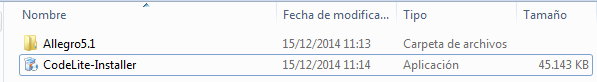
\includegraphics[scale=0.6]{img/Installer_1.png}\\
\small{Instal·lador de CodeLite}\\
\end{center}

\newpage
\noindent Al fer click a sobre el fitxer \textit{CodeLite-Installer.exe} ens apareixerà la següent finestra:

\begin{center}
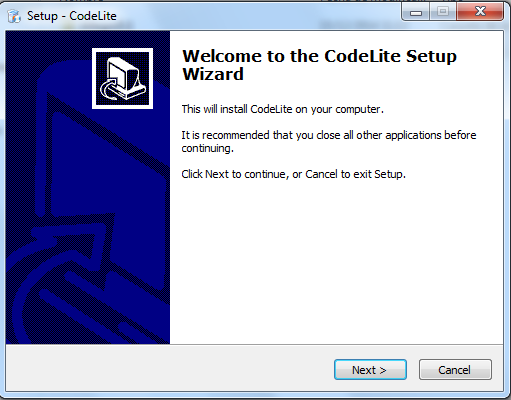
\includegraphics[scale=0.4]{img/Installer_2.png}\\
\small{Finestra de benvinguda}\\
\end{center}

\noindent En aquesta finestra de benvinguda només ens caldrà prémer el botó \textit{Next} per poder prosseguir amb la instal·lació del programa.

\begin{center}
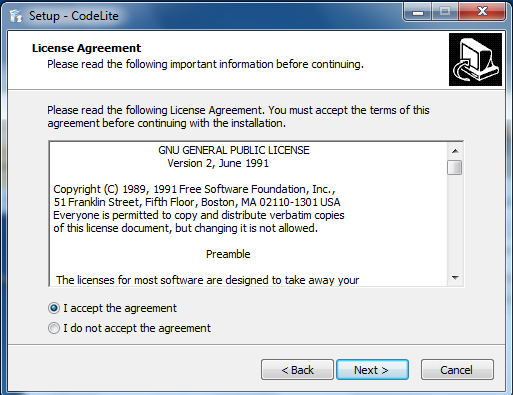
\includegraphics[scale=0.4]{img/Installer_3.png}\\
\small{Finestra de condicions legals}\\
\end{center}

\newpage

\noindent A la finestra anterior, se'ns mostren les condicions legals d'ús del programa. Haurem d'acceptar-les tot marcant la casella \textit{I accept the agreement} i desrpés fer click al botó \textit{Next}. \\\\
\noindent Tot seguit, ens apareixerà una finestra que ens demanarà el directori on instal·lar el programa. Si no teniu cap preferència especial, es recomana deixar el que ja ve pre-establert i prémer el botó \textit{Next} per continuar. A continuació es deixa una imatge de l'aspecte visual de la finestra de selecció del directori d'instal·lació:

\begin{center}
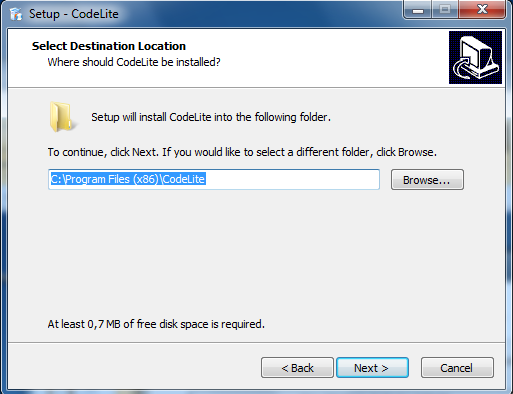
\includegraphics[scale=0.4]{img/Installer_4.png}\\
\small{Finestra de selecció de directori d'instal·lació}
\end{center}

\noindent Un cop fet això, la següent finestra mostrarà un llistat de paquets instal·lables que es poden incloure com a extres amb CodeLite. D'aquests paquets només ens caldrà seleccionar els següents:

\begin{itemize}
	\item CodeLite IDE (Editor + Plugins)
	\item GCC 4.8.1-3 (TDM/GCC) ful (gcc/g++/gdb/WinAPI)
\end{itemize}

\newpage

\noindent Per tant, la finestra de selecció de paquets hauria de quedar de la següent manera:

\begin{center}
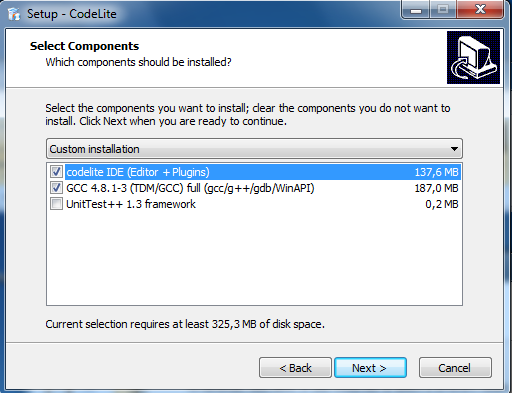
\includegraphics[scale=0.4]{img/Installer_5.png}\\
\small{Finestra de selecció de paquets}
\end{center}

\noindent Per passar a la següent finestra, farem click al botó \textit{Next}.\\\\
La següent finestra que ens apareixerà serà la que ens permetrà seleccionar el directori on instal·lar el compilador de C associat amb CodeLite. La configuració per defecte ja ens serveix i, per tant, farem click al botó \textit{Next} per passar a la següent finestra sense canviar cap paràmetre. A continuació es deixa una imatge que reflexa l'aspecte visual de la finestra de selecció de directori del compilador.

\begin{center}
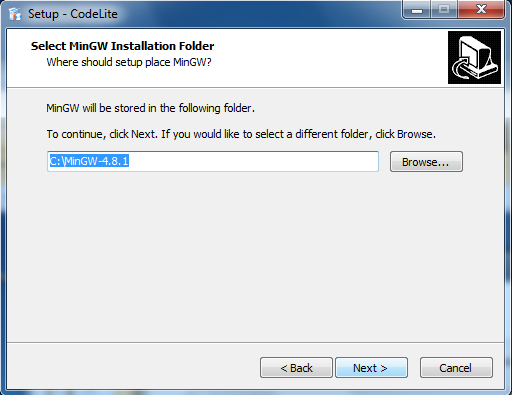
\includegraphics[scale=0.4]{img/Installer_6.png}\\
\small{Finestra de selecció del directori del compilador}
\end{center}

\newpage

\noindent La següent finestra que ens apareixerà ens permet triar el nom de la carpeta del menú Inicio que contindrà els accessos directes al programa. És una configuració al gust de l'usuari, però no hauria de ser necessari canviar-hi cap paràmetre. A continuació es mostra una imatge il·lustrativa d'aquesta finestra en la qual, si no es vol modificar cap dada, només hauríem de fer click al botó \textit{Next}:

\begin{center}
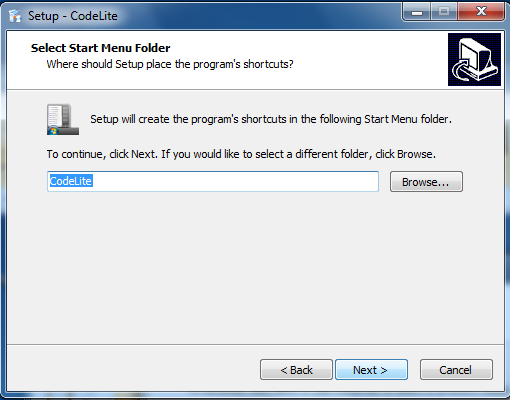
\includegraphics[scale=0.5]{img/Installer_7.png}\\
\small{Finestra de configuració del Menú Inicio}
\end{center}

\noindent Un cop fet, el programa ens mostrarà una altre finestra on haurem de seleccionar les següents opcions:

\begin{itemize}
	\item Create a desktop icon
	\item Create a QuickLaunch icon
\end{itemize}

\newpage

\noindent Aquestes dues opcions faran que el programa aparegui automàticament l'escriptori del nostre ordinador i al menú "Quick Launch". A continuació es mostra una imatge de com hauria de quedar la finestra:

\begin{center}
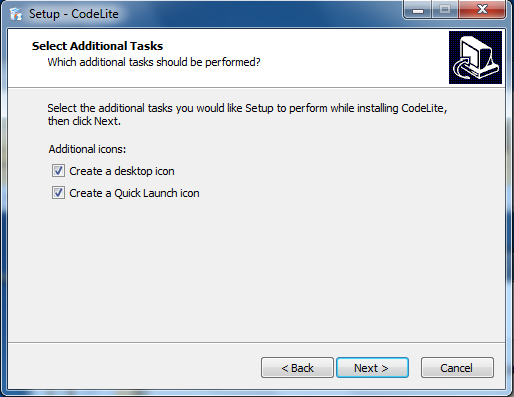
\includegraphics[scale=0.5]{img/Installer_8.png}\\
\small{Finestra de selecció de creació d'icones}
\end{center}

\noindent La següent finestra ens mostrarà un resum de les opcions seleccionades al llarg de tot l'assistent a mode de resum. Per continuar, farem click al botó \textit{Next} tal i com es mostra a la següent imatge:

\begin{center}
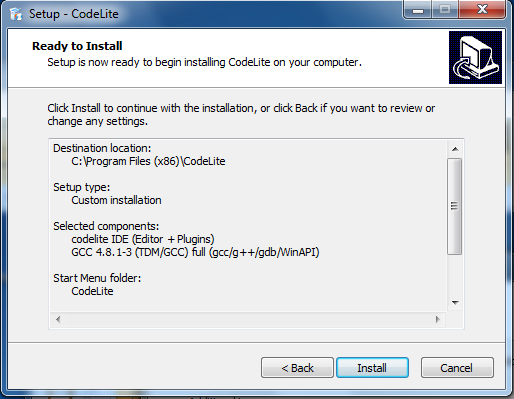
\includegraphics[scale=0.5]{img/Installer_9.png}\\
\small{Finestra resum d'instal·lació}
\end{center}

\noindent Tot seguit, ens apareixerà la finestra amb la barra de progrés de la instal·lació. Haurem d'esperar a que aquesta es completi per poder seguir endavant. La finestra hauria de ser semblant a la que es mostra a continuació:

\begin{center}
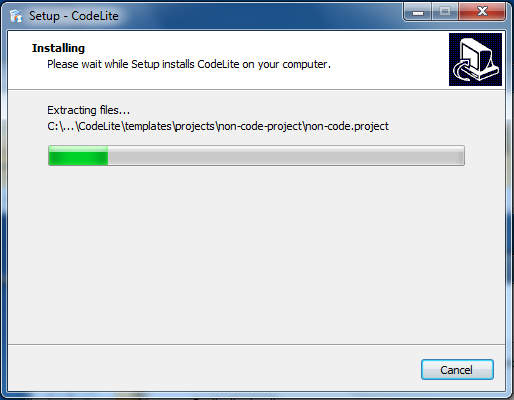
\includegraphics[scale=0.5]{img/Installer_10.png}\\
\small{Finestra de progrés de la instal·lació}
\end{center}

\noindent Un cop completada la barra de progrés, ens apareixerà la següent finestra on només haurem de fer click al botó \textit{Finish}.

\begin{center}
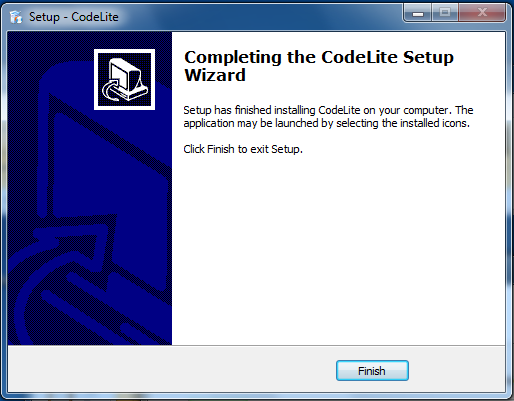
\includegraphics[scale=0.5]{img/Installer_11.png}\\
\small{Finestra de finalització de l'instal·lador}
\end{center}

\noindent Un cop fet tot aquest procés, ja podem procedir a instal·lar Allegro 5.1 com una extensió del compilador de Code-Lite. Per fer-ho, anirem a la carpeta on hem descomprimit el fitxer \textit{.zip} que ens hem descarregat a l'apartat 2 d'aquest document i accedirem a la carpeta \textit{Allegro5.1} tal i com es mostra a continuació:

\begin{center}
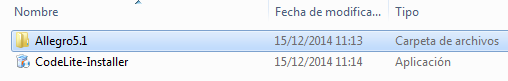
\includegraphics[scale=0.6]{img/Allegro5_Source.png}\\
\small{Carpeta fitxer descomprimit}
\end{center}

\noindent Un cop a dins, veurem tres carpetes. Les haurem de seleccionar totes tres i copiar-les tal i com es veu a la imatge següent:

\begin{center}

\includegraphics[scale=0.6]{img/Origin_Folder.png}\\
\small{Carpeta fitxer descomprimit}
\end{center}

\begin{center}
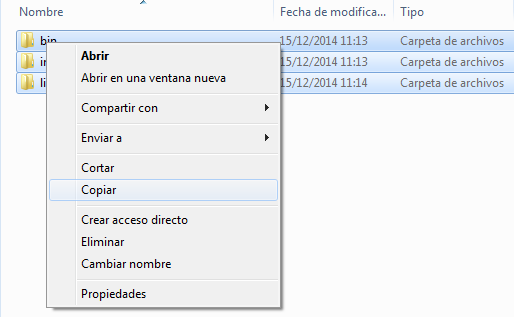
\includegraphics[scale=0.5]{img/Copy.png}\\
\small{Continguts carpeta Allegro 5.1}
\end{center}

\noindent Tot seguit, ens desplaçarem a la carpeta del compilador que acabem d'instal·lar amb CodeLite. Si no hem canviat la carpeta per defecte, aquest s'hauria de trobar a la següent ruta:

\begin{verbatim}
	C:/MinGW-4.8.1
\end{verbatim}

\noindent Per accedir a aquesta carpeta, anirem a \textit{Equipo}, \textit{Disco Local C:} i entrarem a la carpeta \textit{MinGW-4.8.1} tal i com es veu a continuació:\\

\begin{center}

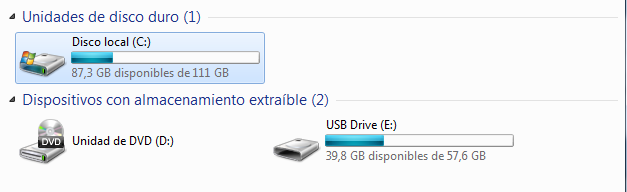
\includegraphics[scale=0.4]{img/Equipo.png}\\
\small{Finestra Equipo}\\

\vfill

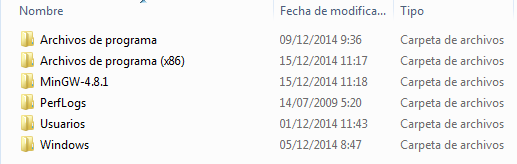
\includegraphics[scale=0.4]{img/MinGW.png}\\
\small{Finestra Disco Local C}\\

\vfill

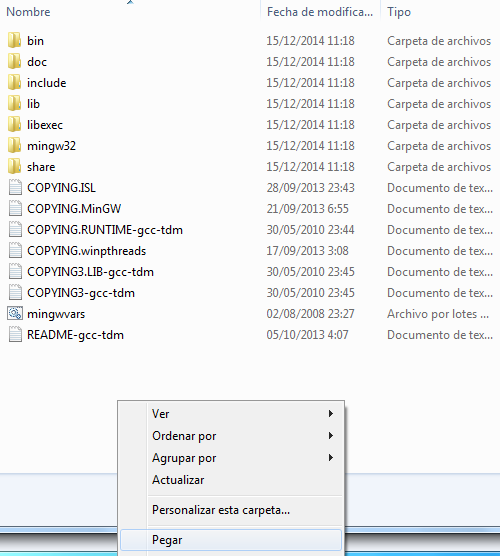
\includegraphics[scale=0.4]{img/Paste.png}\\
\small{Finestra carpeta MinGW}\\
\end{center}


\newpage

\noindent Al moment de fer l'acció de \textit{Pegar} veurem que se'ns mostra la següent finestra:

\begin{center}

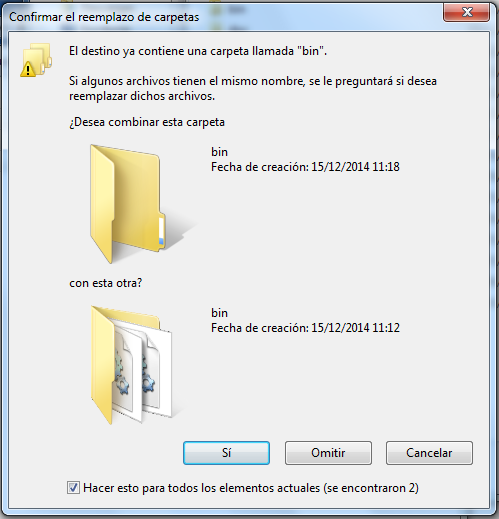
\includegraphics[scale=0.5]{img/Merge.png}\\
\small{Finestra de combinar}\\
\end{center}

\noindent En aquesta finestra, seleccionarem l'opció \textit{Sí} i esperarem a que es completi el procés de copia. Un cop finalitzat, ja haurem instal·lat CodeLite i Allegro5.1 al nostre ordinador.

\newpage
\section{Configuració bàsica del programa}
Per poder deixar enllestit el programa, ens caldrà realitzar unes últimes configuracions. Per fer-les, obrirem el programa fent doble click sobre l'icona
de l'escriptori.

\begin{center}
	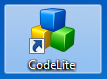
\includegraphics[scale=0.5]{img/Icono.png}\\
	\small{Icona de l'escriptori}
\end{center}

\noindent Un cop obert el programa, ens apareixerà la finestra de selecció del compilador que tindrà el següent aspecte:

\begin{center}
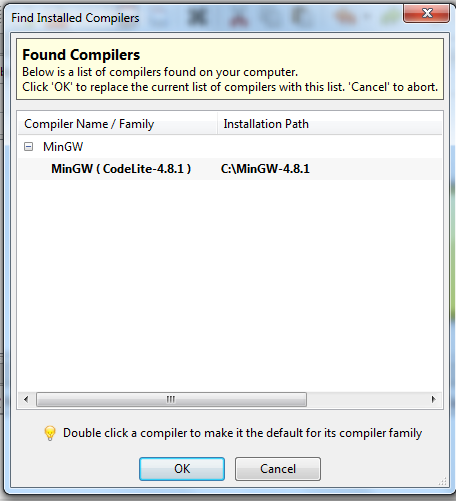
\includegraphics[scale=0.5]{img/Select_Compiler.png}\\
\small{Selecció del compilador}
\end{center}

\noindent En aquesta finestra és \textbf{MOLT} important que seleccioneu el compilador MinGW (CodeLite-4.8.1) encara que n'apareguin d'altres, ja que és l'únic que te la llibreria Allegro instal·lada.

\newpage
Un cop fet click al botó \textit{OK} ens apareixerà la següent finestra:

\begin{center}
	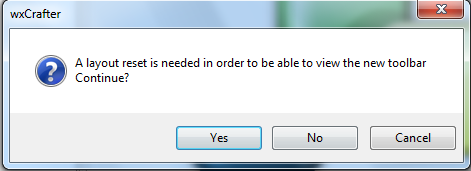
\includegraphics[scale=0.6]{img/Reload.png}\\
	 \small{Finestra de recàrrega de la interfície}
\end{center}

\noindent L'únic que haurem de fer serà fer click al botó \textit{Yes} i ja tindrem el CodeLite preparat per començar a programar.
\end{document}